\section*{Redes de N rendijas}

\item Una onda plana monocromática de longitud de onda $\lambda$ incide normalmente sobre una red de transmisión plana formada por $N$ rendijas de ancho $b$ y período $d$.
Suponiendo que la teoría corresponde a una descripción exacta del fenómeno: 
\begin{enumerate}
	\item Analice la distribución de irradiancia sobre la pantalla y grafíquela.
	\item Calcule:
	\begin{enumerate}
		\item La posición angular de las líneas espectrales (¿a qué máximos corresponden?), y su irradiancia.
		\item El número de mínimos de interferencia entre dos líneas espectrales, por ende, ¿cuántos máximos secundarios hay?
		\item El ancho angular de las líneas espectrales.
		\item El máximo orden observable. 
	\end{enumerate}
	\item Discuta: 
	\begin{enumerate}
		\item ¿Qué aproximación hace en los ángulos?
		\item La dependencia de los parámetros con el número de rendijas y con la densidad de rendijas. 
	\end{enumerate}
\end{enumerate}



\item Sobre la red del problema anterior incide la superposición de dos ondas planas monocromáticas de longitudes de onda $\lambda$ y $\lambda+\Delta\lambda$.
\begin{enumerate}
	\item Calcule la dispersión angular, el poder resolvente, y el máximo del mismo.
	\item Grafique la irradiancia sobre la pantalla. 
	\item Recalcule el problema anterior para una incidencia distinta de la normal, y discuta si existe alguna ventaja al trabajar de esa manera. 
\end{enumerate}



\item 
\begin{minipage}[t][3.3cm]{0.6\textwidth}
Se tiene un dispositivo como el que se muestra en la figura, formado por una red dispuesta entre dos lentes. La red es iluminada por dos fuentes $S_1$ y $S_2$ que emiten luz con la misma irradiancia, pero con longitudes de onda $\lambda_1$ y $\lambda_2$ respectivamente.
Se sabe que la red es de rendijas, pero no se conocen su número \(N\), ancho \(b\) o período de la red \(d\).
\end{minipage}
\begin{minipage}[c][0cm][t]{0.35\textwidth}
	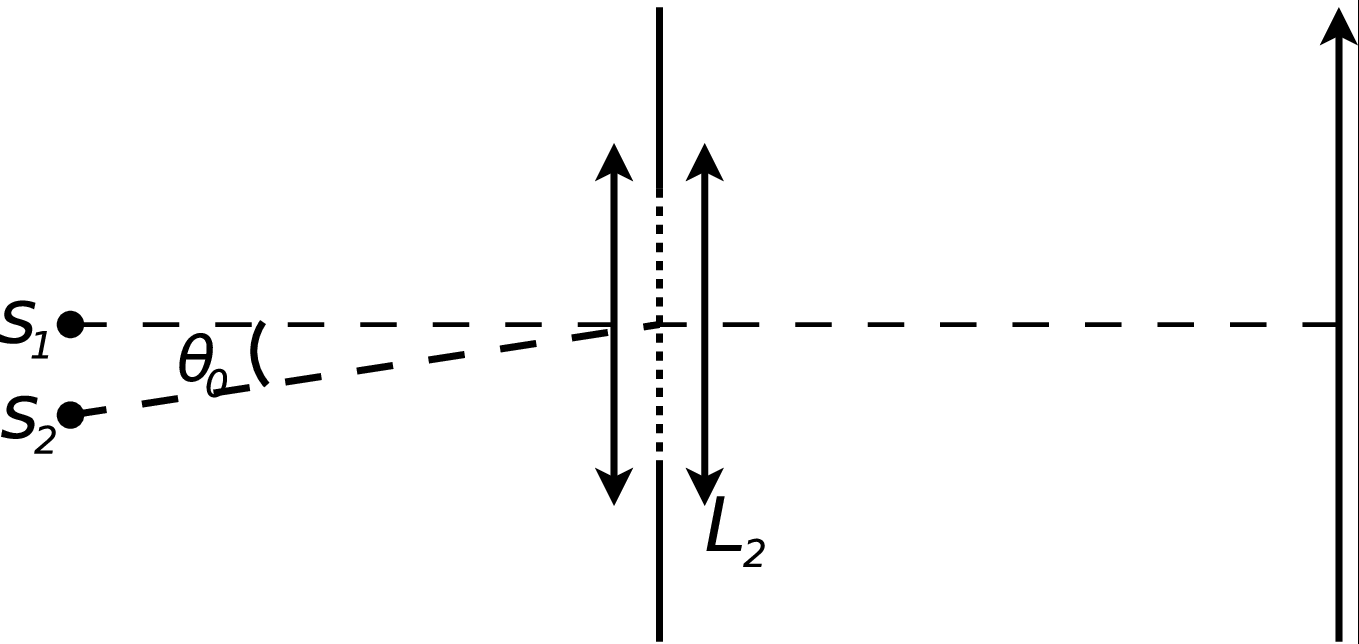
\includegraphics[width=\textwidth]{ej5-43}
\end{minipage}
Para poder caracterizarla, se realizan observaciones de la figura de difracción--interferencia producida en el plano de observación.
A partir de lo cual se logra determinar que:
\begin{itemize}
	\item El orden \num{-1} de interferencia correspondiente a $\lambda_2$ se encuentra una distancia $a_0= \SI{0.1}{\milli\metre}$ por encima del orden \num{+1} correspondiente a $\lambda_1$. 
	\item El ancho de la campana de difracción correspondiente a $\lambda_1$ es $d_0= \SI{10}{\centi\metre}$.
\end{itemize}
Realizar lo siguiente con los datos: distancia focal de la lente $L_2 = \SI{3}{\metre}$; $\lambda_1 = \SI{4000}{\angstrom}$ y $\lambda_2 = \SI{5000}{\angstrom}$.
\begin{enumerate}
	\item Dar la expresión para la distribución de irradiancia que se observa en la pantalla y justificar por qué la escribe así.
	Hacer un gráfico muy cualitativo de dicha distribución (que dé una idea básica de lo que se va a observar).
	\item Determinar las posiciones angulares de todos los ceros de interferencia y difracción. 
	\item Determinar las posiciones de los órdenes de interferencia.
	\item Encontrar los parámetros de la red $b$ y $d$. 
	\item Ambos órdenes (¡cuidado; se trata de órdenes diferentes!) están suficientemente separados entre sí, según el criterio de Rayleigh.
	Hallar una cota	para $N$. 
\end{enumerate}
